\documentclass[a4paper, UKenglish]{lipics-v2016}
 
\usepackage{microtype}
\usepackage[table]{xcolor}
\usepackage{booktabs}
\usepackage{makecell}
\usepackage{ucs}

\usepackage{newfloat}
\DeclareFloatingEnvironment[fileext=lol, name=Listing]{listing}

\usepackage{standalone}

\usepackage{tikz}
\usetikzlibrary{arrows}
\usetikzlibrary{calc}
\usetikzlibrary{decorations.pathreplacing}
\usetikzlibrary{positioning}
\usetikzlibrary{matrix}

\usepackage{enumitem}

\bibliographystyle{plainurl}

\usepackage[firstpage]{draftwatermark}
\SetWatermarkText{\hspace*{6.3in}\raisebox{5in}{
\includegraphics[scale=0.1]{aec-badge-ecoop}}}
\SetWatermarkAngle{0}

\newcommand{\code}[1]{{\ttfamily #1}}

\newcommand{\const}{{\bfseries \ttfamily const}}

\newcommand*\circled[1]{\tikz[baseline=(char.base)]{
            \node[shape=circle,draw,inner sep=2pt] (char) {#1};}}

\newcommand{\wtc}{write-through-\const{}}
\newcommand{\wstc}{writes-through-\const{}}
\newcommand{\wtcq}{write-through-\const{}-qualifier}
\newcommand{\wstcq}{writes-through-\const{}-qualifier}
\newcommand{\wtcqs}{write-through-\const{}-qualifiers}
\newcommand{\wstcqs}{writes-through-\const{}-qualifiers}
\newcommand{\Wstcqs}{Writes-through-\const{}-qualifiers}
\newcommand{\wtcqd}{write-through-\const{}-qualified}
\newcommand{\wstcqd}{writes-through-\const{}-qualified}

% Author macros::begin %%%%%%%%%%%%%%%%%%%%%%%%%%%%%%%%%%%%%%%%%%%%%%%%%%%%%%%%%
\title{C++ \const{} and Immutability: An Empirical Study of Writes-Through-\const{}}

\author[1]{Jon Eyolfson}
\author[2]{Patrick Lam}
\affil[1]{University of Waterloo\\
  Waterloo, ON, Canada\\
  \texttt{jeyolfso@uwaterloo.ca}}
\affil[2]{University of Waterloo\\
  Waterloo ON, Canada\\
  \texttt{patrick.lam@uwaterloo.ca}}
\authorrunning{J. Eyolfson and P. Lam}

\Copyright{Jonathan Eyolfson and Patrick Lam}

%% mandatory: Please choose ACM 1998 classifications from
%% http://www.acm.org/about/class/ccs98-html . E.g., cite as
%% "F.1.1 Models of Computation". 
\subjclass{D.3.3 Language Constructs and Features}
% mandatory: Please provide 1-5 keywords
\keywords{empirical study, dynamic analysis, immutability}
% Author macros::end %%%%%%%%%%%%%%%%%%%%%%%%%%%%%%%%%%%%%%%%%%%%%%%%%%%%%%%%%%%

%Editor-only macros:: begin (do not touch as author)%%%%%%%%%%%%%%%%%%%%%%%%%%%%%%%%%%
\EventEditors{John Q. Open and Joan R. Acces}
\EventNoEds{2}
\EventLongTitle{42nd Conference on Very Important Topics (CVIT 2016)}
\EventShortTitle{CVIT 2016}
\EventAcronym{CVIT}
\EventYear{2016}
\EventDate{December 24--27, 2016}
\EventLocation{Little Whinging, United Kingdom}
\EventLogo{}
\SeriesVolume{42}
\ArticleNo{23}
% Editor-only macros::end %%%%%%%%%%%%%%%%%%%%%%%%%%%%%%%%%%%%%%%%%%%%%%

\begin{document}

\maketitle

\begin{abstract}
The ability to specify immutability in a programming language is a powerful tool
for developers, enabling them to better understand and more safely transform
their code without fearing unintended changes to program state.
The C++ programming language allows developers to specify a form of immutability
using the \const{} keyword.
In this work, we characterize the meaning of the C++ \const{} qualifier and
present the ConstSanitizer tool, which dynamically verifies a stricter form of
immutability than that defined in C++: it identifies \const{} uses that are
either not consistent with transitive immutability, that write to mutable
fields, or that write to formerly-\const{} objects whose \const{}-ness has been
cast away.

We evaluate a set of 7 C++ benchmark programs to find \wstc{}, establish root
causes for how they fail to respect our stricter definition of immutability, and
assign attributes to each write (namely: synchronized, not visible,
buffer/cache, delayed initialization, and incorrect).
ConstSanitizer finds 17 archetypes for writes in these programs which do not
respect our version of immutability.
Over half of these seem unnecessary to us.
Our classification and observations of behaviour in practice contribute to the
understanding of a widely-used C++ language feature.
\end{abstract}

\section{Introduction}
Immutability is an important concept that simplifies reasoning about programs
and eases software maintenance.
Most importantly, immutability circumscribes possible side effects, 
so that (in some cases) a user of a function may avoid closely
examining the implementation of the function and its callees.
One concrete application of immutability is: if a developer knows that a library
function does not modify one of its arguments (including transitive arguments),
then they know that it is safe to call that library function with that argument
from multiple threads, as the function only requires read access to its
argument.

C++~\cite{programming-langauges-cpp-n3690} is a popular language that allows
programers to specify immutability using \const{}\footnote{Some of our
discussion also applies to C, but we focus
on C++ in this paper.}.
C++ experts such as Meyers recommend judicious use of
``\const{}-correctness''~\cite{effective-cpp} in C++ codebases.
It is generally clear when developers could use \const{}, but not (in
non-obvious cases) when they should use \const{}.

We distinguish between two uses of C++'s \const{} qualifier:
\const{}-qualified global/stack objects, whose data may never change (i.e.
immutable objects), and \const{}-qualified references/pointers to objects (i.e.
read-only references~\cite{lncs-2013-7850-potanin}).
(For now, assume that there are no casts that remove \const{} qualifiers and no
\texttt{mutable} storage class specifiers; these language features violate
immutability.)
An \emph{immutable object}'s fields may never change, and mutable references to
that object may never be created.
A \emph{read-only reference}, on the other hand, only guarantees immutability
for accesses through qualified references.
An object with a read-only reference to it may still be mutated through other,
mutable, references.
C++ enforces a shallow immutability guarantee (also known as bitwise \const{})
for writes through the read-only reference: while it is illegal to reassign the
fields of such an object, any referents of fields may change.
We expand on this in
Section~\ref{section:background}.

C++'s type system admits several workarounds to \const{}'s supposed
immutability guarantees.
Much research defines type qualifiers similar to C++ \const{}, but with stronger
guarantees.
These type systems do not have any holes in the type system, such as
unsafe casts.
Furthermore, they not only ensure that the field values do not change, but also ensure
that objects referenced through fields also do not change (i.e. deep, or
transitive, immutability; again, see Section~\ref{section:background} for more
details).

On the other hand, our industrial contacts have indicated that, in their
codebases, \const{} has been used to deter new developers from modifying certain
variables.
Such variables may be modified by an experienced developer ready to assume the
consequences~\cite{fang:_person}.
In such cases, \const{} serves an advisory role, but does not provide any
guarantees.

Our goal is to explore the space of possible meanings for immutability
declarations in C++ and to examine what guarantees developers appear to be
expecting in practice.
We developed a tool, ConstSanitizer, that instruments programs to identify
source locations that modify \const{}-qualified objects, using more restrictive
semantics than guaranteed by C++.
ConstSanitizer monitors \wstc{}, i.e. writes performed on
\const{}-qualified objects or references, either transitively (which is allowed
in C++), or through C++'s \const{} escape hatches.
To better understand \const{} usage in practice, we ran ConstSanitizer on a
benchmark suite and manually classified all \wstc{}.

Specifically, the goal of this work is to answer the following research
questions:
\vspace*{-0.25em}
\begin{enumerate}
  \item[({\bf RQ1})] Do developers perform shallow and transitive \wstc{}? \\[0.2em]
        \hspace*{1em}
        \begin{minipage}{4.5in} (Answer: Yes to both.) \end{minipage}~\\[-1em]

  \item[({\bf RQ2})] How do developers \wtc{}? \\[0.2em]
        \hspace*{1em}
        \begin{minipage}{4.5in}
          (Answer: By directly writing to fields of \const{}-qualified objects
          and through transitive writes; both are about equally common.)
        \end{minipage}~\\[-0.5em]
  \item[({\bf RQ3})] Why do developers write to fields of \const{}-qualified objects?
        \\[0.2em]
        \hspace*{1em}
        \begin{minipage}{4.5in}
          (Answer: Buffers and delayed initialization were important reasons,
          but over half the time, we couldn't find any clear reason motivating
          developers' decisions to write through \const{}.)
        \end{minipage}~\\[-0.5em]
\end{enumerate}

Section~\ref{section:conclusion} presents our detailed answers to these questions.

\vspace*{1em}
Our contributions include:
\vspace*{-0.25em}
\begin{itemize}
  \item the design and implementation of a novel dynamic analysis for C++ that
        detects \wstcqd{} variables (both shallow and transitive);
  \item an empirical study of \const{} usage (including \wstcqs{}) on a suite of
        7 C++ benchmarks; and,
  \item based on the empirical study, a novel classification of \wstcqs{} in the
        wild according to a root cause and a set of attributes.
\end{itemize}


\section{Motivating Example}
\label{section:motivating-example}
\documentclass[tikz]{standalone}

\usepackage{fontspec}

\usetikzlibrary{arrows}
\usetikzlibrary{calc}
\usetikzlibrary{decorations.pathreplacing}
\usetikzlibrary{positioning}
\usetikzlibrary{matrix}

\usepackage{fontspec}

\begin{document}

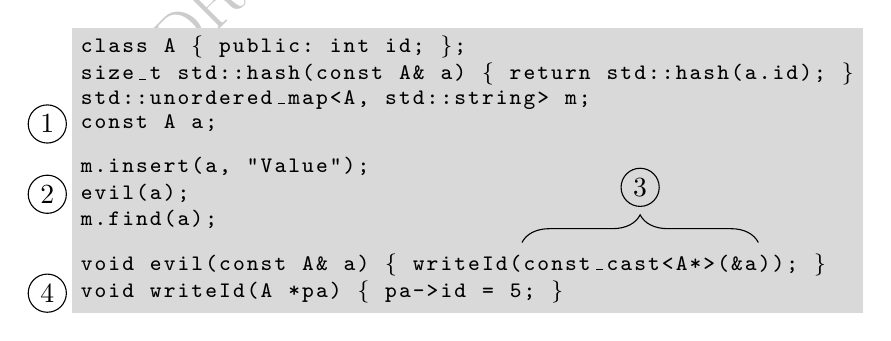
\begin{tikzpicture}
  [node distance=5mm, >=stealth',
  every node/.style={font=\footnotesize},
  every matrix/.style={fill=black!15, inner sep=1mm, row sep=0.5mm,
                        matrix of nodes, nodes in empty cells,
                        minimum height=0.5em, minimum width=.5em,
                        nodes={anchor=base, inner sep=0, font=\ttfamily\footnotesize}}]

  \matrix (snippet) {
c & l & a & s & s &   & A &   & \{ &   & p & u & b & l & i & c & : &   & i & n & t &   & i & d & ; &   & \} & ; &   &   &   &   &   &   &   &   &   &   &   &   &   &   &   &   &   &   &   &   &   &   &   &   &   &   &   &   \\
s & i & z & e & \_ & t &   & s & t & d & : & : & h & a & s & h & ( & c & o & n & s & t &   & A & \& &   & a & ) &   & \{ &   & r & e & t & u & r & n &   & s & t & d & : & : & h & a & s & h & ( & a & . & i & d & ) & ; &   & \} \\
s & t & d & : & : & u & n & o & r & d & e & r & e & d & \_ & m & a & p & < & A & , &   & s & t & d & : & : & s & t & r & i & n & g & > &   & m & ; &   &   &   &   &   &   &   &   &   &   &   &   &   &   &   &   &   &   &   \\
c & o & n & s & t &   & A &   & a & ; &   &   &   &   &   &   &   &   &   &   &   &   &   &   &   &   &   &   &   &   &   &   &   &   &   &   &   &   &   &   &   &   &   &   &   &   &   &   &   &   &   &   &   &   &   &   \\
  &   &   &   &   &   &   &   &   &   &   &   &   &   &   &   &   &   &   &   &   &   &   &   &   &   &   &   &   &   &   &   &   &   &   &   &   &   &   &   &   &   &   &   &   &   &   &   &   &   &   &   &   &   &   &   \\
m & . & i & n & s & e & r & t & ( & a & , &   & " & V & a & l & u & e & " & ) & ; &   &   &   &   &   &   &   &   &   &   &   &   &   &   &   &   &   &   &   &   &   &   &   &   &   &   &   &   &   &   &   &   &   &   &   \\
e & v & i & l & ( & a & ) & ; &   &   &   &   &   &   &   &   &   &   &   &   &   &   &   &   &   &   &   &   &   &   &   &   &   &   &   &   &   &   &   &   &   &   &   &   &   &   &   &   &   &   &   &   &   &   &   &   \\
m & . & f & i & n & d & ( & a & ) & ; &   &   &   &   &   &   &   &   &   &   &   &   &   &   &   &   &   &   &   &   &   &   &   &   &   &   &   &   &   &   &   &   &   &   &   &   &   &   &   &   &   &   &   &   &   &   \\
  &   &   &   &   &   &   &   &   &   &   &   &   &   &   &   &   &   &   &   &   &   &   &   &   &   &   &   &   &   &   &   &   &   &   &   &   &   &   &   &   &   &   &   &   &   &   &   &   &   &   &   &   &   &   &   \\
v & o & i & d &   & e & v & i & l & ( & c & o & n & s & t &   & A & \& &   & a & ) &   & \{ &   & w & r & i & t & e & I & d & ( & c & o & n & s & t & \_ & c & a & s & t & < & A & * & > & ( & \& & a & ) & ) & ; &   & \} &   &   \\
v & o & i & d &   & w & r & i & t & e & I & d & ( & A &   & * & p & a & ) &   & \{ &   & p & a & - & > & i & d &   & = &   & 5 & ; &   & \} &   &   &   &   &   &   &   &   &   &   &   &   &   &   &   &   &   &   &   &   &   \\
  };

  \node [left of=snippet-4-1, circle, draw, font=\normalsize, inner sep=2pt]
        {1};
  \node [left of=snippet-7-1, circle, font=\normalsize, inner sep=2pt, draw]
        {2};
  \draw[decorate, decoration={brace, amplitude=10pt}]
       ($ (snippet-10-33.north west) + (0, 2mm) $)
       -- node[above, yshift=10pt+1mm, circle, font=\normalsize, inner sep=2pt, draw]
       {3}
       ($ (snippet-10-49.north east) + (0, 2mm) $);
  \node [left of=snippet-11-1, circle, font=\normalsize, inner sep=2pt, draw]
        {4};
\end{tikzpicture}

\end{document}


\section{Meaning of \const{} in C++}
\label{section:background}
As discussed earlier, the C++ \const{} keyword allows programmers to declare,
in some sense, that a value should not change.
In this section, we explain the specific guarantees that C++ provides, and we
present the deep immutability variant of these guarantees that we verify.

\subparagraph*{Meaning of \const{} on C++ primitive and pointer types.}

The meaning of \const{} in C++ is an extension of its meaning in C.
We start by describing the common meaning of \const{} across C and C++, applying
to primitive and pointer types.
In these languages, the \const{}-ness of a memory location depends on the
qualifiers of the variable through which the location is accessed; our
motivating example illustrated a change in \const{}-ness through a cast, in
function \texttt{evil()}, that is allowed by both C and C++.

Developers may \const{}-qualify primitive types such as \code{\texttt{int}},
resulting in immutable object types like \code{\const{} \texttt{int}}.
When variable $v$ has primitive \const{}-qualified type, the C++ type system
prevents developers from assigning to $v$ after its definition; i.e. it
prevents writes to $v$.
In this case, \const{} behaves like \texttt{final} in Java, which also
prevents re-assignment.

For pointer types, such as \code{\texttt{int *}}, developers may
\const{}-qualify both the pointee and pointer type.
The \const{} qualifier applies to the type directly to the left of it; if there
is nothing to the left, then \const{} applies to the right.
If a variable has type \code{\texttt{int *}\const{}}, developers may not change
the address value of the variable (where it points to), but they may dereference
the location and change the value it points to.
A different type is \code{\texttt{int} \const{} \texttt{*}} (also known as
\code{\const{} \texttt{int} \texttt{*}}), which allows the address value to
change, but not the value pointed-to by the variable.
This type represents a read-only reference.
The \const{} qualifier may also apply to both the pointer and pointee types
(\code{\texttt{int} \const{} \texttt{*} \const{}}), which prevents writes to
both the address value and the value pointed-to.
If all pointers to a value are read-only references, then the value pointed-to
is immutable.
C++ references can be thought of as \const{}-qualified pointers; a developer may
not write to the reference address value.
However, in contrast with pointers, developers cannot cast away reference
address value \const{}-ness and re-assign the address value; this property is
enforced by the language.

\begin{listing}[!htb]
  \caption{The \const{} qualifier may apply to C++ member functions.}
  \label{listing-const-background}
  \centering
  \includestandalone{listing/const-background}
\end{listing}

\subparagraph*{Meaning of \const{} on C++ object types.}
We continue by exploring the meaning of \const{} in C++-specific contexts.
When a C++ object type is \const-qualified,
the developer may only call member functions declared with a
\const{} qualifier.

\const{}-qualifying a member function has two effects.
First, \const{}-qualifying a member function allows it to be called on a
\const{}-qualified receiver object.
Furthermore, inside the function, the type qualifiers of the receiver object's
fields are treated as \const{}.

Conceptually, each C++ class provides two
interfaces: the \const{}-qualified interface and the non-\const{} qualified
interface.
A \const{}-qualified reference is meant to be a read-only
reference, although C++ enforces no guarantees.
One of our goals is to evaluate whether read-only guarantees hold in practice.
When an object has non-\const{} type, then the developer may call all methods on
that object\footnote{There is a small exception: on a non-\const{} object, the
developer cannot call \const{}-qualified methods that are hidden due to
overloading by a non-\const{}-qualified method of the same signature.}.
On the other hand, when an object has \const{} type, then the developer may only
call methods on that object that are \const{}-qualified.

Consider class \texttt{Pointish}, defined in
Listing~\ref{listing-const-background}.
As written, the developer could call all methods on a non-\const{}-qualified
object of type \texttt{Pointish}.
On the other hand, the developer may only call the \texttt{getX()} method on a
\const{}-qualified \texttt{Pointish} object.

The second effect of \const{}-qualifying a function changes the type qualifiers of
fields inside the function.
In our example, field \texttt{x} becomes \texttt{int}
\const{} within \const{}-qualified member functions.
The compiler successfully compiles \texttt{getX()}, since there are no
writes to \texttt{x} or \texttt{y}.
But, if \texttt{setX()} was \const{}-qualified, the compiler would refuse to
compile the code, since the type of \texttt{x} would be treated as \const{}
\texttt{int} and \texttt{setX()} contains a write to that variable.

In C++, without using \const{} escape hatches, developers may re-assign
fields in non-\const{} qualified methods and may not re-assign fields in
\const{}-qualified methods.
In all methods, developers are permitted to mutate state outside of
re-assignment (through references or pointers).
This type of immutability is referred to as \emph{shallow immutability}.

A C++ \const{}-qualified stack/global object would be considered a shallow
\emph{immutable object}.
That is, without escape hatches, developers cannot create non-\const{}
references (including through pointers) to such a \const{}-qualified object.
However, as we discuss next, developers may indeed remove the \const{} qualifier
on references to the \const{}-qualified object.
Therefore, C++ does not strongly enforce the concept of an immutable object.

\subparagraph*{Working around \const{} restrictions.}
Practical type systems appear to require escape hatches.
C++'s escape hatches for \const{} include casting (the sole
escape hatch in C) and \texttt{mutable}.
Also, C++ \const{} does not specify deep immutability.
ConstSanitizer dynamically observes executions to
monitor uses of escape hatches and deep immutability.

Most type systems permit casting between types.
C-style casts (\code{(const A)a}) and C++ \texttt{const\_cast}s can
add or remove \const{} qualifiers.
\const{} manipulation may also occur through unions and
\texttt{reinterpret\_cast}s.
ConstSanitizer ignores casts, instead using the declared type of
a variable or function argument.
When there is a mismatch between variable and function argument types, we
persist all \const{} information.

For \const{} member functions, ``\texttt{mutable}'' instructs the
compiler to not add the implicit \const{} type qualifier otherwise imposed on
fields inside those functions.
In Listing~\ref{listing-const-background}, if \texttt{x} were instead
declared as \code{\texttt{mutable int x}}, then \texttt{setX()} could be
\const{}-qualified and still compile.
ConstSanitizer would then report the write to field \texttt{x} whenever
\texttt{setX()} was called on a \const{} receiver object, as we consider the
write to be a breach of that object's immutability.

ConstSanitizer goes beyond C++'s guarantees with respect to transitivity.
Consider again Listing~\ref{listing-const-background}.
Field \texttt{y} has type \code{int *}; within a \const{}-qualified member
function, its type is \code{int *const}.
C++ therefore prevents writes to \texttt{y} inside a \const{}-qualified member
function.
However, it does not prevent writes to \texttt{*y} without further explicit
markup (i.e. \code{int const *const}).
We call writes to locations like \texttt{*y} \emph{transitive writes}.

C++ only guarantees shallow immutability---that is, field values
directly stored in a \const{}-qualified class do not change.
If a field has pointer type, C++ ensures that the pointer value does not change,
but does not guarantee anything about the value pointed to.
ConstSanitizer verifies \emph{deep immutability} through transitive writes, and
enables us to answer the empirical question of whether extant programs preserve
deep immutability or not.


\section{Technique}
\label{section:technique}
Our ConstSanitizer tool generates instrumented code which, when executed,
prints out notifications about \wstcqs
\footnote{We previously implemented a static analysis which was an unpublishable
          dead end. Most of its reported violations required calling context to
          make sense of; context-sensitive interprocedural analysis would thus
          be required to get meaningful results.
          Static counts of mutables and const casts were too overwhelming.
          Furthermore, imprecision due to pointers made its results unusable.}.
ConstSanitizer builds upon LLVM~\cite{llvm} and was inspired by existing
sanitizers including AddressSanitizer~\cite{2012-usenix-serebryany} and
MemorySanitizer~\cite{2015-cgo-stepanov}.

We implemented ConstSanitizer by extending the \texttt{clang} frontend and
adding instrumentation passes on \texttt{llvm} bitcode.
The instrumented code calls hooks in our modified version of \texttt{llvm}'s
\texttt{compiler-rt} runtime library.
Figure~\ref{figure:overview-src-to-obj} depicts our processes for compiling
instrumented code.
Plain text indicates inputs and outputs; outlined boxes indicate existing
software components; and light gray boxes indicate our modifications.

We first describe our modifications to the \texttt{clang} frontend.
When the developer enables ConstSanitizer (using a command-line flag), our
frontend adds metadata about initialization expression extents to the bitcode.
This metadata notifies the \texttt{llvm}-level instrumentation about
source-level constructs that would otherwise be lost in translation to bitcode.

Specifically, we modified \texttt{clang}'s bitcode generator at variable
declaration statements.
At statements of the form \code{type var = expr} we mark the instructions
making up \code{expr} so that our \texttt{llvm}-level
instrumentation can ignore them.
The rationale for ignoring those writes is that the primary user-visible write
from a \texttt{clang} declaration statement is to \code{var}, on the
left-hand side.
We empirically observed that other writes within \code{expr} are almost always
initialization writes to \code{var}, which ought
not to be reported even if \code{var} is \const{}.
Although a programmer may include explicit (side-effecting) writes within
\code{expr}, we ignore such writes to eliminate the false positives
that otherwise occur due to initialization writes.

\begin{figure}
  \centering
  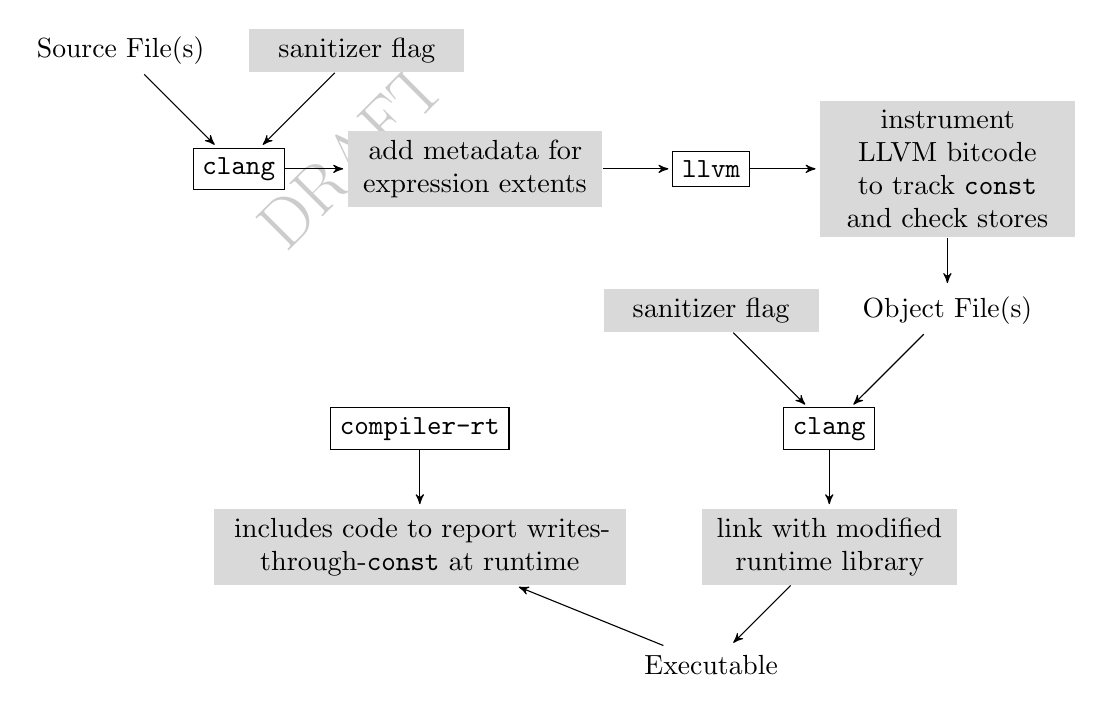
\begin{tikzpicture}[->,>=stealth',shorten >=0.5mm,node distance=3cm]
    \node (src) {Source File(s)};
    \node (clang) [xshift=1.5cm, yshift=-0.5cm, draw, node distance=1cm,
                   below of=src]
          {\texttt{clang}};
    \node (flag) [fill=black!15, text width=2.5cm, text centered,
                  right of=src]
          {sanitizer flag};
    \node (clang-mod) [fill=black!15, text centered, text width=3cm,
                       right of=clang]
          {add metadata for expression extents};
    \node (llvm) [rectangle, draw, right of=clang-mod] {\texttt{llvm}};
    \node (llvm-mod) [fill=black!15, text centered, text width=3cm,
                      right of=llvm]
          {instrument LLVM bitcode to track \const{} and check stores};
    \node (obj) [node distance=1.8cm, below of=llvm-mod] {Object File(s)};

    \path (src) edge (clang)
          (flag) edge (clang)
          (clang) edge (clang-mod)
          (clang-mod) edge (llvm)
          (llvm) edge (llvm-mod)
          (llvm-mod) edge (obj);
    \node (clang2) [xshift=-1.5cm, yshift=-0.5cm, draw, node distance=1cm,
                   below of=obj]
          {\texttt{clang}};
    \node (flag) [fill=black!15, text width=2.5cm, text centered,
                  left of=obj]
          {sanitizer flag};
    \node (clang-mod) [yshift=1.5cm, fill=black!15, text centered,
                       text width=3cm, below of=clang2]
          {link with modified runtime library};
    \node (compiler-rt-mod) [xshift=-1.5cm,fill=black!15, text centered,
                             text width=5cm, node distance=3.7cm,
                             left of=clang-mod]
          {includes code to report \wstc{} at runtime};
    \node (compiler-rt) [rectangle, draw, node distance=1.5cm,
                         above of=compiler-rt-mod]
          {\texttt{compiler-rt}};
    \node (exe) [xshift=-1.5cm, node distance=1.5cm, below of=clang-mod]
          {Executable};

    \path (obj) edge (clang2)
          (flag) edge (clang2)
          (clang2) edge (clang-mod)
          (clang-mod) edge (exe)
    (compiler-rt) edge (compiler-rt-mod)
    (exe) edge (compiler-rt-mod);
  \end{tikzpicture}
  \caption{ConstSanitizer generates instrumented LLVM bitcode which reports
           writes through \const{} qualifiers at runtime.}
  \label{figure:overview-src-to-obj}
\end{figure}

We use \const{}-ness information as provided by declarations,
rather than implementing a taint-based approach.
Listing~\ref{listing-false-negative-example} shows a false negative caused by
our approach.
The debugging information for \texttt{y} gives shadow value
$(\texttt{00})_2$.
Hence, on the write through \texttt{y}, we do not report a \wtc{},
because we do not propagate \const{}-ness information from variable
initializers.
One might expect this write to trigger a report since \texttt{y} aliases
the read-only reference \texttt{x}.
(We report a write if the cast is part of a function argument.)

\begin{listing}[ht]
  \caption{C++ source code showing a false negative due to expression handling.}
  \label{listing-false-negative-example}
  \centering
  \includestandalone{listing/false-negative-example}
\end{listing}

Most of our instrumentation lives in a custom \texttt{llvm} pass that
generates code to track \const{}-ness of the program's values.
The instrumentation manipulates shadow values to track \const{} qualifiers at
every instruction that generates a pointer value.
The \const{} information relies on type tables from DWARF 4 debugging
information.
In \texttt{llvm}, this includes all variables in functions---all local
variables are allocated on the stack and are pointers.

Our dynamic analysis returns (as one might expect) no false positives, since it
observes program executions.
However, it depends on the accuracy of the debugging information and
metadata, which it uses to identify which variables are \const{}-qualified in
the source and to identify initialization expression extents.
We ran into one false positive in our results which we believe is the result of
the metadata being invalidated between LLVM passes.
Throughout the remainder of the section, we point out a couple of cases where
our analysis must approximate intended \const{}-ness because actual
\const{}-ness information does not exist.

\begin{table}[!b]
  \caption{Shadow values encode available \const{}-ness restrictions on
           variables.}
  \label{tab:shadow-value-example}
  \centering
  \begin{tabular}{@{}lrlr@{}} % \toprule
    \renewcommand{\arraystretch}{1.2}
    \textbf{Declaration} & \textbf{Shadow value} & \textbf{Example statement}
    & \textbf{Allowed} \\ \midrule
    \code{int x} & $(0)_2$ & \code{x = 5} & $\checkmark$ \\
    \arrayrulecolor{black!10} \hline
    \code{\const{} int x} & $(1)_2$ & \code{x = 5} & $\times$ \\
    \arrayrulecolor{black!30} \hline

    \code{int * x}  & $(00)_2$ & \code{x = y} & $\checkmark$ \\
    && \code{*x = 55} & $\checkmark$ \\ \arrayrulecolor{black!10} \hline

    \code{int *\const{} x} & $(01)_2$ & \code{x = y} & $\times$ \\
    && \code{*x = 55} & $\checkmark$ \\ \hline

    \code{\const{} int * x} & $(10)_2$ & \code{x = y} & $\checkmark$ \\
    (or \code{int \const{} * x}) && \code{*x = 55} & $\times$ \\ \hline

    \code{\const{} int *\const{}} & $(11)_2$ & \code{x = y} & $\times$ \\
    (or \code{int \const{}  *\const{}}) && \code{*x = 55} & $\times$  \\
    \arrayrulecolor{black}
  \end{tabular}
\end{table}

\subparagraph*{Structure of shadow values.}

A shadow value consists of $n$ bits tracking \const{}-ness (where $n$ is the word length of
the processor architecture).
Each bit represents whether a pointer or pointee has a \const{}
qualifier or not.
The rightmost bit represents the \const{} qualifier of the value itself.
Bits to the left (if the value is a pointer) represent what the pointer
transitively points to.
Our encoding supports pointers up to $n-1$ levels deep on $n$-bit processors
(64 for our experiments).
Figure~\ref{figure:shadow-values} depicted our encoding of shadow values, while
Table~\ref{tab:shadow-value-example} shows how shadow values represent
sample \const{}-ness settings and corresponding writes allowed.

\subparagraph*{Shadow value computation.}

We next describe how we create and propagate shadow values.
Our ConstSanitizer instrumentation dynamically propagates shadow values
representing \const{} qualifiers through a program's instructions.
Our goal is to monitor 1) writes to \texttt{mutable} fields; 2) locations where
\const{} has been cast away; and 3) transitive writes, to pointees of fields,
through \const{} references.
Table~\ref{tab:technique-summary} summarizes the analysis rules.

\begin{table}[!b]
  \caption{Dynamic analysis rules showing computation of shadow value for result
           \texttt{\%1}.}
  \label{tab:technique-summary}
  \centering
    \small
  \begin{tabular}{l p{8cm}}
    \textbf{Instruction} & \textbf{New shadow value} \\
    \midrule
    \texttt{\%1 = alloca ...} &
      from \const{} qualifiers in debugging
      information, consistent with Figure~\ref{figure:shadow-values}.
      \\[0.5em]
    \texttt{\%1 = getelementptr \%2} &
      by logically shifting left \texttt{\%2}'s shadow value once for each
      dereference this instruction represents.

      \textbf{if field access}: check \const{} qualifier of base object; for
      (immutable) \const{} base objects, new shadow value is all ones, otherwise all zeros.
      \\[0.5em]
    \texttt{\%1 = call(\%2)} &
      loaded from return shadow value in Thread-Local Storage (TLS).

      \textbf{for pointer arguments \texttt{\%2}:} also write shadow values to
      appropriate TLS slots for the function call; if the call and argument are
      marked as ignored, write all zeros for the shadow value for the argument.
      \\[0.5em]
    \texttt{\%1 = phi}/\texttt{select} \texttt{...} &
      carry out same operation on shadow value operands.
      \\[0.5em]
    \texttt{\%1 = bitcast \%2} &
      from the shadow value for \texttt{\%2}, if compatible; \\ & otherwise all
      zeros.
      \\[0.5em]
    \texttt{\%1 = load \%2} &
      logical shift right of \texttt{\%2}'s shadow value.
      \\[0.5em]
    \texttt{store \%2, \%1} &
      check rightmost bit of shadow value for \texttt{\%1}, report \wtc{} if
      set. (Only applies if the instruction not ignored as an initializer.)

      \textbf{if \texttt{\%2} is function argument:} load shadow value for
      \texttt{\%2} from TLS, left shifted once. New shadow value is bitwise OR
      of shifted value with previously computed shadow value for \texttt{\%1}.

      \textbf{if \texttt{\%2} is ``this'' function argument:} same steps as
      above, except skip the bitwise OR step.

      \textbf{if \texttt{\%2} is ``this'' function argument for destructor:} shadow
      value for \texttt{\%1} is $(00)_2$.
      \\[0.5em]
    \texttt{\%1 = extractelement}
       &
       all zeros.\\
    \texttt{\%1 = extractvalue}\\
    \texttt{\%1 = inttoptr} \\
    \texttt{\%1 = landingpad}
      \newline
      \\
  \end{tabular}
\end{table}

\texttt{llvm} bitcode uses \texttt{alloca} instructions to introduce new pointer
values.
Our \texttt{llvm} pass instruments each \texttt{alloca} instruction with the
appropriate shadow value, as extracted from the type information in the source
code, using standard \texttt{clang} debug information.

Ultimately, our instrumentation verifies the behaviour of \texttt{store}
instructions.
Recall that we exclude \texttt{store} instructions that come from the right-hand
side of a declaration statement.
For all other \texttt{store}s, we check whether the operand---the location being
written-to---represents a \const{}-qualified type.
The rightmost bit of the shadow value provides this information.
If that bit is 1, an execution of this \texttt{store} instruction is a write to
a \const{}-qualified location.
We insert a call to our runtime library to check the value of the bit and to
report a \wtc{} if the bit is 1.
(We later discuss a special case for store instructions where the value being
stored is a function argument.)

Conversely, \texttt{load} instructions return a pointer that represents a single
pointer dereference.
To compute the returned shadow value, we right shift the operand's shadow value.

\texttt{llvm}'s \texttt{getelementptr} (GEP) instruction accesses arrays and
fields of objects.
This instruction preserves type safety through dereferences in the compilation
process and is a safe alternative to directly generating pointer arithmetic
code.
Our instrumentation performs a logical shift right by one bit for every pointer
dereference implied in the GEP instruction.
Our treatment of GEP implicitly handles transitive immutability as follows: when
a GEP accesses an object field, and the containing object is \const{}-qualified,
we generate a shadow value as if the field had a \const{} qualifer on every type
for the contained field.
This treatment implies checks for transitive immutability; generating a
non-\const{} shadow value here would generate the same bitwise immutability
checks for \const{} as specified by the C++ standard.

Our instrumentation propagates \const{}-ness information (in
shadow values) alongside references to that location.
In C++, access restrictions to a location depend on whether the
program is accessing that location through a \const{} reference or not.
Therefore, in the presence of casts and pointer arithmetic, there is no ground
truth about the \const{}-ness of the resulting references and we must make a
reasonable under-approximation as to \const{}-ness.

We next discuss casting-related \texttt{llvm} instructions.
The \texttt{bitcast} instruction converts a value into a specified type.
If a program converts a pointer between equally-indirected pointer types, then
we copy the old shadow value to the result.
(C++ \const{}-casts do not appear at LLVM bitcode level, nor
do the component of a C-style cast that manipulates \const{}-ness.
ConstSanitizer preserves declared \const{}-ness for such variables.)
Otherwise, we choose to assume that the instruction's result has no \const{}
qualifiers.
We make this assumption in all cases for the \texttt{inttoptr} instruction,
which represents pointer arithmetic not handled by the GEP instruction, as well
as for \texttt{extractvalue} and \texttt{extractelement}.

Our instrumentation stores shadow values for function calls' arguments and
return values using thread local storage (TLS).
In the straightforward case, we store shadow values for pointer arguments in
TLS slots reserved for each argument.
However, we ignore pointer arguments' \const{} qualifiers if the call and the
argument are both part of a variable declaration.
As for (pointer) return values: if a function was instrumented by our tool, then
we read the shadow value from the appropriate TLS slot.
We also store a mutable shadow value in the return value TLS slot, in case the
function had not been instrumented by our tool.
Our instrumentation either reads the approximation or, if applicable, the actual
return value generated by the called function.
In the presence of callbacks from uninstrumented code back to instrumented code,
our instrumentation may use stale shadow values and report extraneous results
based on these stale shadow values.

We have a special case for store instructions where the value stored is a
function argument, as mentioned above.
Consider a store instruction ``\texttt{store value, location}''.
We compute the shadow value for ``\texttt{location}'' as follows.
First, we get the shadow value for ``\texttt{value}'' from the TLS.
Then, we adjust this shadow value to be compatible with the type of
``\texttt{location}'': our encoding requires one logical shift to match the type
of ``\texttt{value}'' to that of ``\texttt{location}''.
We bitwise OR the shadow value for ``\texttt{location}'' previously computed
(from an \texttt{alloca} instruction) with the shifted value to get the new
shadow value for ``\texttt{location}''.
This preserves \const{} qualifiers of the original argument and of the local
variables in the function.

There are two further special sub-cases for store instructions and function
arguments for (i) method and (ii) destructor calls.
Listing~\ref{listing-llvm-example} illustrates sub-case (i).
Here, \texttt{foo()} is declared \const{}.
The compiler will hence treat \texttt{this} as \const{} within \texttt{foo()}.
However, for our dynamic analysis, we want to detect writes based on the
\const{}-ness of \texttt{this} from the caller; in method \texttt{bar()} in
Listing~\ref{listing-llvm-example}, receiver object \texttt{nc} for
\texttt{foo} is not \const{}, so we do not want to report the call's (transitive) store
to \texttt{x}.
\texttt{foo}'s method arguments appear as ``\texttt{value}'' operands of
\texttt{store} instructions while the ``\texttt{location}'' is an
\texttt{alloca} within the function.
We set the shadow value of the associated \texttt{alloca} instruction to the
value of the argument after applying a logical shift left by one (since it's a
pointer).
This treatment properly ignores \const{} qualifiers added due to callee
method signatures.

For sub-case (ii), destructors, we do not want to report any writes through
\texttt{this} as the object no longer exists after the call (so that writes to
the object aren't visible in any case).
We handle this case by simply assuming that the \texttt{this} argument is
mutable.
For all other arguments, we do a bitwise OR between the \texttt{alloca} shadow
value and the argument shadow value logically shifted left by one, which
maintains all \const{} qualifiers.

\begin{listing}[ht]
  \caption{C++ source code showing calls to method \texttt{foo()} (with
           its definition and associated LLVM bitcode) from \const{} context
           \texttt{cc} and non-\const{} context \texttt{nc}.}
  \label{listing-llvm-example}
  \centering
  \includestandalone{listing/llvm-example}
\end{listing}

\subparagraph*{Shadow value computation example.}

Listing~\ref{listing-llvm-example} presents the C++ source code for
\code{C::foo}, a \const{} qualified method, and the associated LLVM bitcode.
Consider the \code{bar} function, which calls \code{foo} twice, first with
mutable (i.e. non-\const{}) receiver object \texttt{nc} and then with \const{}
receiver object \texttt{cc}.
Within \code{bar}, the shadow value of \texttt{nc} is $(0)_2$ and the shadow
value of \texttt{cc} is $(1)_2$.
Our instrumentation assigns shadow values for each LLVM instruction with a
pointer result. We instrument \code{C::foo} as follows:

\begin{itemize}
  \item The first instruction, \texttt{alloca}, stores its result in
        \texttt{\%1}.
        Since it is an \texttt{alloca} instruction, we obtain its shadow value
        from \texttt{clang} debugging information.
        The associated shadow value is $(10)_2$: in this \const{}-qualified
        method, the type of \code{this} is that of a \const{} pointer to the
        containing class, \code{\const{} C *}.
  \item At the \texttt{store} instruction, without special handling, we would
        load the shadow value of argument \texttt{\%this} from the TLS;
        logically shift left the shadow value by one to account for the fact
        that we are performing a \texttt{store} to memory allocated for that
        argument; and bitwise OR the resulting shadow value with the original
        shadow value for \texttt{\%1}.
        In our example, whether the receiver object is \texttt{cc} or
        \texttt{nc}, the shadow value for \texttt{\%1} is $(10)_2$.
  \item Next, we obtain the shadow value for the result of the \texttt{load},
        \texttt{\%2}.
        As \texttt{\%2} returns a pointer, we shift \texttt{\%1}'s (the
        operand's) shadow value right by one, giving a shadow value of $(1)_2$.
  \item Next, the \texttt{getelementptr} instruction results in a pointer to the
        class's \texttt{x} field.
        Our instrumentation of \texttt{getelementptr} could produce two
        different shadow values, depending on the instruction's operand.
        In this case, \texttt{\%2} is a \const{} object, and the resulting
        shadow value for a fully \const{}-qualified \texttt{x} field is
        $(11)_2$.
  \item Next, we obtain the shadow value for the \texttt{load} result
        \texttt{\%4} using the same technique as for \texttt{\%2}.
        The resulting shadow value is $(1)_2$.
  \item Finally, we insert a check at the \texttt{store} instruction.
        In this case, the least significant bit of the shadow value associated
        with location (\texttt{\%4}) is 1.
        Therefore we would dynamically report a \wtc{} at the write to field
        \texttt{x} of the \const{} method.
\end{itemize}

For methods, this instrumentation is not enough.
We only want to report a \wtc{} for the call with \const{} receiver object even
though both objects call the same static method.
Before the call to \code{foo}, our instrumentation stores the shadow value of
the receiver object in its TLS slot.
Our instrumentation of \code{foo} looks for \texttt{store} instructions that use
the receiver object and recomputes the shadow value of the location.
Here, we load the shadow value from its TLS slot and shift left
to match the type of the expected shadow value of \texttt{\%1}.
For \texttt{nc}'s call, this shadow value is $(00)_2$.
Since \code{foo} is a method, we ignore the original shadow value of
\texttt{\%1} ($(10)_2$) and overwrite it with new shadow value
$(00)_2$.
Following the remaining steps in \code{foo} as above, the shadow value of
\texttt{\%4} is now $(0)_2$ and we do not report a \wtc{}.
In the \texttt{cc} case, we would follow the same steps, but instead report a
\wtc{}, because the shadow value would be $(10)_2$.


\section{Classification of \wstc{}}
\label{section:classification}
One of our contributions is a careful analysis of the \const{} usages detected
by our ConstSanitizer dynamic analysis tool.
We propose a classification for \wstcqs{} along 2 axes.
We manually assigned each write 1) a single cause, from a set of common root
causes; and 2) a set of additional attributes. This classification distills our
empirical observations about \const{} use in practice.

\begin{table}[ht!]
  \caption{Root causes of writes through \const{} and our symbols for these causes.}
  \label{table:root-cause-reference}
  \centering
  \begin{tabular}{l c}
    \textbf{Root Cause} & \textbf{Symbol} \\
    \midrule
    Write to mutable field         & M \\
    Transitive write               & T \\
    Write after casting a \const{} qualifier away & C \\
  \end{tabular}
\end{table}

\noindent Table~\ref{table:root-cause-reference} lists all of the root causes
for \wstc, along with a one-letter abbreviation that
we will use in Section~\ref{section:results}'s tables.
ConstSanitizer detects such writes and reports them to the user.
The causes are:

\begin{itemize}
  \item mutable field (M): the program writes to a \texttt{mutable}-labelled
        field of a \const{} object.
        \begin{center}
          \includestandalone{listing/mutable-field}
        \end{center}
        \texttt{mutable} permits method \texttt{mutator()} to
        write to field \texttt{x} even though it is a \const{} method, which
        would ordinarily prevent (at compile-time) writes to fields of the
        \texttt{this} object.

  \item transitive write (T): the program writes through a field of a \const{}
        object.
        \begin{center}
          \includestandalone{listing/transitive-write}
        \end{center}
        \const{}-qualified method \texttt{transitiveWrite()} writes to
        field \texttt{x} of the \texttt{this} object.
        While the \const{} qualifier prevents mutation of the \texttt{x} field,
        it does not prevent transitive writes of the memory pointed to by
        \texttt{x}.

  \item casting away const (C): the program writes through a pointer which has
        previously been \const{} but whose \const{}-ness has been cast away
        using a \code{const\_cast} or C-style cast.
        \begin{center}
          \includestandalone{listing/const-cast}
        \end{center}
        The write in \texttt{writeToArg()} mutates the value pointed-to by
        \texttt{x} while \texttt{x} is \const{}-qualified.
        ConstSanitizer reports \wstcqs{} whose \const{}-ness has been
        cast away, using the \const{}-ness of the most recent
        declared type for the value.
\end{itemize}

\vspace*{-1em}
\begin{table}[ht!]
  \caption{Observed common attributes of writes through \const{} and corresponding
           symbols.}
  \label{table:classification-reference}
  \centering
  \begin{tabular}{l c}
    \textbf{Attribute} & \textbf{Symbol} \\
    \midrule
    Write is synchronized & S \\
    Write is not visible  & N \\
    Write is to a buffer/cache & B \\
    Write is delayed initialization & D \\
    Write is incorrect & I \\
  \end{tabular}
\end{table}

Table~\ref{table:classification-reference} summarizes our attributes for \wstcqs.
We assigned attributes to writes based on our understanding of the code.
Writes may have multiple attributes; for instance, a
write in our Protobuf benchmark is B \& N \& S.
The attributes are:

\begin{itemize}
  \item synchronized (S): indicates that the write is always protected by a
        lock.
        This attribute is often required under the C++11 standard: all types
        that are shared between threads and that may be used with the standard
        library must be either bitwise const, which is clearly not the case when
        we witness a write, or else protected against concurrent
        accesses~\cite{sutter13:_gotw_solut}.
        The following example, from Protobuf, is synchronized using Google mutex
        primitives.
        \begin{center}
          \includestandalone{listing/synchronized}
        \end{center}
  \item not visible (N): indicates that the result of the write is never
        externally visible (e.g. private and with no accessor methods; may be
        accessed in the same translation unit).
        Often occurs in the context of testing-related counters.
        \begin{center}
          \includestandalone{listing/not-visible}
        \end{center}
  \item to a buffer/cache (B): indicates that the write is of a derived value
        which can be computed from other currently-available state.
        Such writes are often optimizations.
        \begin{center}
          \includestandalone{listing/buffer}
        \end{center}
  \item delayed initialization (D): indicates that the write initializes state
        not initialized in the constructor or its transitive
        callees.
        Writes with this attribute could have also occurred
        in the constructor, but the written value was not yet
        available.
        Failure to call a delayed initialization method would lead to undesired
        behaviours (or lack of desired behaviours).
        \begin{center}
          \includestandalone{listing/delayed-initialization}
        \end{center}
  \item incorrect (I): indicates that the write appeared to violate the
        \const{}-ness of the object.
\end{itemize}

Note that S/N/B/D writes are not necessarily errors and do not necessarily
violate immutability properties.
We thus chose the word ``attribute'' to suggest that S/N/B/D indicate an
incidental property of a \wtc.
If the code containing the writes is properly written, an object with an
S/N/B/D \wtc{} can still appear to be immutable to the client, assuming all
references to that object are read-only.
A write with attribute I, however, is a client-visible violation of \const{}.


\section{Results}
\label{section:results}
We evaluated our ConstSanitizer tool on 7 C++ software projects, plus 1 C project.
We attempted to choose significant benchmarks using these
guidelines:

\begin{enumerate}
  \item must span a range of application areas: applications and libraries; small,
        medium, and large projects; interactive and non-interactive;
  \item are used by the community: the Google projects are the most popular on
        GitHub; the applications are popular among FOSS users; contributor-group
        sizes vary from a core group to a large community; and,
  \item must extensively use \const{} constructs.
\end{enumerate}

\noindent
A ConstSanitizer report indicates that a write that would not be allowed under
deep immutability occurred through a read-only reference.
Such writes are allowed under C++ semantics.
They are only a departure from the \const{} semantics that we experiment
with (i.e. deep immutability with no casts and no mutable).
Our experiments classify \wstc{} observed in actual \const{}-using programs.
Classifying these writes provides us valuable insight about \const{} usage in
practice, which will guide future work.

Our approach was to modify the project's build system to use our tool and to
disable optimizations.
We then ran the project's test suite, when available, and collected output from
our instrumentation.
Using this output we categorized the writes that we found, assigning root causes
and attributes.
Along with the number of static locations of writes that we found
(\textbf{bolded}), we also report the number of dynamic occurrences of each
write over observed executions.
All else being equal, dynamic counts can help prioritize \wstc{}, with
more-frequent locations to be investigated first.
We refer to these dynamic occurrences of writes as ``occurrences'' in the
sequel.
Table~\ref{table:projects} summarizes our benchmark projects.

\begin{table}[!htb]
  \centering
  \caption{We ran our experiments across 7 C++ (and 1 C) software projects;
           ConstSanitizer introduces a build slowdown of
           1.05$\times$--1.40$\times$ across all projects.}
  \label{table:projects}
  \begin{tabular}{l l r l r}
    & \textbf{Name} & \textbf{Version} & \textbf{Description}
    & \makecell[r]{\textbf{Build} \\ \textbf{Slowdown}}\\
    \midrule
    C++ & Protobuf & 2.6.1 & Serialization framework & 1.40$\times$\\
    C++ & LevelDB & 1.18 & Key/value database & 1.05$\times$\\
    C++ & fish shell & 2.2.0 & UNIX shell & 1.32$\times$\\
    C++ & Mosh (mobile shell) & 1.2.5 & SSH replacement & 1.26$\times$\\
    C++ & LLVM TableGen & 3.7.0 & Domain-specific generator & ---\phantom{\- $\times$} \\
    C++ & Tesseract & 3.04.00 & OCR engine & 1.10$\times$\\
    C++ & Ninja & 1.6.0 & Build system & 1.20$\times$\\
    C & Weston & 1.9.0 & Wayland compositor & 1.28$\times$\\
  \end{tabular}
\end{table}

We recorded relative overhead introduced by our instrumentation with respect to
both building and testing times on the longest-running projects, Protobuf and
LevelDB.
Table~\ref{table:projects} includes build slowdowns induced by our tool, which
ranged between 1.05$\times$ and 1.40$\times$.
Our tool caused a 3.3$\times$ slowdown and 1.3$\times$ slowdown in test
execution times for Protobuf and LevelDB respectively.
The remaining projects were either interactive, or did not have long enough
running test suites to get meaningful results.
We do not any report LLVM TableGen numbers because we built it (with
instrumentation) as part of the LLVM build process and were not able to build
the executable separately.

\subsection{Protobuf}

Protobuf is Google's serializing framework for structured data, consisting of
about 214~000 lines of C++ code.
We analyzed version 2.6.1 of Protobuf by running its test suite, which contains
5 tests.
Table~\ref{table:protobuf-violations} summarizes the Protobuf results.
ConstSanitizer found {\bf 76} static write locations (and 127~644 occurrences).
We describe 5 archetypes for these writes.
An archetype is a group of writes that we judged to be similar; the writes may
happen at different source locations.

\begin{table}[!htb]
  \centering
  \caption{Protobuf shows 5 archetypes for {\bf 76} writes through \const{} resulting in 127~644
           occurrences.}
  \label{table:protobuf-violations}
  \begin{tabular}{l r r c c}
    \textbf{Archetype} & \textbf{Locations} & \textbf{Occurrences}
                     & \textbf{Root Cause} & \textbf{Attributes} \\
    \midrule
    Generator printer & {\bf 7} & 118464  & T & B \& N \& S \\
    Message cache sizes & {\bf 61} & 7158 & M & B \& S \\
    Source code locations & {\bf 4} & 1898 & T & I \\
    Linked list operations & {\bf 2} & 84 & M & I \& S \\
    Generate initialization \\
    \hspace*{2em}  method & {\bf 2} & 40 &  M & D \& N \& S \\
  \end{tabular}
\end{table}

The ``Generator printer'' archetype occurred most often.
Listing~\ref{listing-protobuf-generator-printer} presents a representative
expanded stack trace.
The function at the top of the listing shows the initiation of the write in
\code{Generator}'s \const-qualified \code{Generate} method.
This method calls \code{PrintTopBoilerplate}, passing a pointer to a mutable
\code{io::Printer}.
Then, \code{Printer}'s \code{WriteRaw} method modifies (root cause T) two fields:
\code{buffer\_} and \code{buffer\_size\_}.
These fields are protected by a lock, act as a buffer, and are not visible
outside the class (which is just a printer).
This archetype also includes other \code{Print}-like calls with different source
locations but a common explanation.

\begin{listing}[!htb]
  \caption{Protobuf's Generator class performing transitive \wtc{} to a Printer
           field.}
  \label{listing-protobuf-generator-printer}
  \centering
  \includestandalone{listing/protobuf-generator-printer}
\end{listing}

The ``Generate initialization method'' archetype is related to ``Generator
printer''.
Listing~\ref{listing-protobuf-generator-lazy} shows this archetype.
The \code{printer\_} field was initialized as seen above.
C++ allows this write due to the \texttt{mutable} specifier.
Another field, \code{file\_}, is lazily initialized as well.
Both of these fields are protected by the same lock, and are not externally
visible outside the class.

\begin{listing}[!htb]
  \caption{Protobuf's Generate initialization method performing lazy initialization.}
  \label{listing-protobuf-generator-lazy}
  \centering
  \includestandalone{listing/protobuf-generator-lazy}
\end{listing}

We show an example of the ``linked list operations'' archetype in
Listing~\ref{listing-protobuf-list}.
Here, the \code{depart} method grabs a lock, and uses a pointer with type
\code{linked\_ptr\_internal \const{} *}, so that the \const{} applies to what is
pointed to, not to the pointer.
The method then modifies the \code{next\_} field of a valid object at the point
indicated by the comment.
The root cause here is \code{mutable}: the \code{next\_} field is declared
\code{mutable linked\_ptr\_internal const* next\_}.
This write is a delayed initialization, not visible, and synchronized.

\begin{listing}[!htb]
  \caption{Protobuf using Google test linked list that writes internally.}
  \label{listing-protobuf-list}
  \centering
  \includestandalone{listing/protobuf-list}
\end{listing}

Listing~\ref{listing-protobuf-cache} shows the ``Message cache
sizes'' archetype.
The write is protected by a lock, and is allowed by C++ because the field is
\texttt{mutable}.
However, this write, while involved with caching, is externally visible.
The method \code{void SetCachedSize(int size) const} enables
external code to modify this field through a \const{}
reference to the containing object.

\begin{listing}[!htb]
  \setlength{\belowcaptionskip}{-1em}
  \caption{Protobuf writing to a message's cached size field.}
  \label{listing-protobuf-cache}
  \centering
  \includestandalone{listing/protobuf-cache}
\end{listing}

Listing~\ref{listing-protobuf-locations} shows the ``Source code locations''
archetype.
The \code{mutable\_leading\_comments} method, which includes ``mutable'' in its
name, is not declared as \const{}, and thus allows writes.
Its implementation writes to the \code{location\_} field; we show an example of
a caller which causes such a write.
The \code{location\_} field is externally-visible, so this is a clearly
incorrect externally-visible transitive write; we assign attribute I.

\begin{listing}[!htb]
  \caption{Protobuf writing to a source location object.}
  \label{listing-protobuf-locations}
  \centering
  \includestandalone{listing/protobuf-locations}
\end{listing}

We also found an archetype involving writing data to a message.
This included 133 unique source locations, occurring 14~638 times in total.
However, the code is heavily inlined and the build system appears to overwrite
optimization settings for this subdirectory.
Manual inspection of the code revealed no obvious writes.
We believe this is a result of optimizations causing invalid debugging
information.
We thus omitted this archetype from Table~\ref{table:protobuf-violations}.

\subsection{LevelDB}

LevelDB (1.18) is Google's lightweight key/value database library, consisting of
approximately 18~000 lines of C++ code.
The test suite contains 23 test drivers.
There were 6 archetypes and also {\bf 6} root source locations for these writes.
These locations contributed to 13~792 occurrences over the test drivers.
Table~\ref{table:leveldb-violations} shows a summary of our findings for
LevelDB.

\begin{table}[!htb]
  \centering
  \caption{LevelDB shows writes from {\bf 6} source locations, with 13~792
           occurrences in total.}
  \label{table:leveldb-violations}
  \begin{tabular}{l  r  c  c }
    \textbf{Location} & \textbf{Occurrences} & \textbf{Root Cause}
    & \textbf{Attributes} \\
    \midrule
    \texttt{db/db\_test.cc:40} & 10311 & T & N \& S \\
    \texttt{util/cache.cc:315} & 2841 & T & B \& S\\
    \texttt{db/snapshot.h:54} & 319 & T & I \\
    \texttt{db/snapshot.h:55} & 319 & T & I \\
    \texttt{helpers/memenv/memenv.cc:274} & 1 & T & I \& S \\
    \texttt{util/testutil.h:42} & 1 & T & N \\
  \end{tabular}
\end{table}

Listing~\ref{listing-leveldb-counter} shows the source location that caused
the majority of the occurrences.
This code extends the \code{RandomAccessFile} class to add an atomic counter
field, \code{counter\_}, that tracks the number of read calls.
The root cause is that \code{counter\_} is a pointer and is transitively written
to.
The reason for this write is test controllability: this class is part of the
test infrastructure.
Yet it must override the monitored call (and thus must be \const{}).
This class is meant for testing purposes only, so we concluded the write was not
visible outside the class---the counter is only used in the testing code.

\begin{listing}[!htb]
  \caption{LevelDB write in \texttt{db\_test.cc:40} incrementing counter tracking
           \# of writes to a file.}
  \label{listing-leveldb-counter}
  \centering
  \includestandalone{listing/leveldb-counter}
\end{listing}

Listing~\ref{listing-leveldb-cache} shows a modification to a caching structure
that generates a new identifier.
This cache is a field, \code{block\_cache}, in \code{options}, which is declared
as \code{const Options\&} in \code{Table::Open}.
The root cause is a transitive write, since the code dereferences a field of a
\const{} object to do the write.
This write is protected by a lock and clearly involved in caching.
However, it appears that other code outside of \code{Options} uses this block
cache.

\begin{listing}[!htb]
  \caption{LevelDB write in \texttt{cache.cc:315} creating a new block cache in
           \code{\const{} Options} object.}
  \label{listing-leveldb-cache}
  \centering
  \includestandalone{listing/leveldb-cache}
\end{listing}

Listing~\ref{listing-leveldb-list} shows a modification of a linked list node
accessed through two pointer dereferences.
This corresponds to both \texttt{snapshot.h} locations shown in the table.
This code modifies the pointers obtained from following its own nodes,
performing a transitive write through a \const{} qualifier.
We do not know why the developers declared \texttt{s} as \const{} since it is
also destroyed at the end of the method. In any case, we assigned attribute I.

\begin{listing}[!htb]
  \caption{LevelDB write in \texttt{snapshot.h} deleting a list element and
           updates pointers.}
  \label{listing-leveldb-list}
  \centering
  \includestandalone{listing/leveldb-list}
\end{listing}

Listing~\ref{listing-leveldb-env} shows a \wtc{} in the \code{InMemoryEnv}
class.
As with the cache, the root cause is a transitive write: in the caller,
\code{options} is declared \code{const Options\&}.
Unlike the caching example, this file isn't involved in caching and appears to
be a visible change to \code{options}.
This write is protected by a lock, giving attribute I \& S.

\begin{listing}[!htb]
  \caption{LevelDB write in \texttt{memenv.cc} changing the environment in
           options object.}
  \label{listing-leveldb-env}
  \centering
  \includestandalone{listing/leveldb-env}
\end{listing}

Listing~\ref{listing-leveldb-test} shows the final \wtcq{} that we found for
LevelDB.
The caller location is the same as in Listing~\ref{listing-leveldb-env} above.
In this case, however, the containing class extends \code{InMemoryEnv} and adds
a field to count the number of errors (for testing purposes only).
Therefore we attribute this write as being not visible---it is only used in
tests.

\begin{listing}[!htb]
  \caption{LevelDB write in \texttt{testutil.h} injecting faults into
           the test suite.}
  \label{listing-leveldb-test}
  \centering
  \includestandalone{listing/leveldb-test}
\end{listing}

\subsection{fish shell}

fish shell (2.2.0) is a UNIX shell providing advanced features, consisting of
approximately 48~000 lines of C++ code.
We compiled the project with our tool and executed an instance of the shell.
Our workload launched the shell and immediately exited.
We found writes from {\bf 4} unique source locations for 98 occurrences in total.
All locations are within the \code{exchange} function.
Listing~\ref{listing-fish} shows this function along with a snippet of
\code{\_wgetopt\_internal} that calls \code{exchange}.
The root cause is that the \const{}-qualified \code{argv}
variable gets cast to non-\const{} and then passed to \code{exchange}.
This write shows that the \const{}-qualifier on \code{argv} is incorrect and
should not be included.

\begin{listing}[!htb]
  \caption{fish shell writing to \const{}-qualified \code{argv} object.}
  \label{listing-fish}
  \centering
  \includestandalone{listing/fish}
\end{listing}

\subsection{Mosh (mobile shell)}

Mosh (mobile shell) (1.2.5) is a remote terminal application that is a
replacement for secure shell (SSH), consisting of about 13~000 lines of C++
code.
Our workload was to launch the mosh server and immediately terminate it.
We found \wstc{} at {\bf 8} unique source locations (432 occurrences).
Listing~\ref{listing-mosh} shows one of the writes.
Mosh parsing code sets a flag to indicate completion.
However, the developers declared the parser action as \const{} in the same
method where they modify it.
The root cause is that the variable \code{handled} is declared \code{public
mutable}.
We believe this is an incorrectly \const{} qualified variable.

\begin{listing}[!htb]
  \caption{Mosh handling terminal action with a \wtc{}.}
  \label{listing-mosh}
  \centering
  \includestandalone{listing/mosh}
\end{listing}

\subsection{LLVM TableGen}

We instrumented LLVM's (3.7) TableGen executable, which uses domain-specific
information to generate files with custom backends.
This part of LLVM consists of approximately 34~400 lines of C++ code.
It is primarily used in building LLVM itself.
We added our instrumentation to the build system and observed reports from an
instrumented version of TableGen executing as part of the build process.
LLVM itself is a large body of code with too many \wstcq{} objects to manually
classify.
In TableGen, we found writes from {\bf 3} unique source locations (282
occurrences).

The handling code for DFAs contains some puzzling writes, shown in
Listing~\ref{listing-llvm-dfa}.
The write immediately follows an instantiation of a \code{\const{} State} object.
The \code{State} class itself is only available in a file's translation unit
(not usable outside the file), which may indicate that the \code{State} is not
intended to be widely used.
\code{State} only contains \const{} methods and all of its fields (except one
explicitly declared \const{}) are mutable.
Since all methods are \const{} there is no difference in callable methods
between non-\const{} and \const{}-qualified access.
In addition, since all other fields are mutable, developers are allowed to
re-assign the same fields in a \const{} method as they would in a non-\const{}
method.
Since only one field doesn't have \texttt{mutable}, developers could achieve the
same effect by making all methods non-\const{}, removing all \texttt{mutable}
specifiers on fields, and changing the one field that did not have
\texttt{mutable} to be \const{} qualified.

\begin{listing}[!htb]
  \caption{LLVM DFA code marks \texttt{State} \const{} for no apparent reason.}
  \label{listing-llvm-dfa}
  \centering
  \includestandalone{listing/llvm-dfa}
\end{listing}

The other write is in the code that computes a sub-register index for code
generation.
Listing~\ref{listing-llvm-subreg} shows the containing method.
The root cause here is that the \code{LaneMask} field is mutable.
The write caches the value.
However, this value is not used in any other methods.

\begin{listing}[!htb]
  \caption{LLVM SubReg writes to a \texttt{mutable} field in a \const{} method.}
  \label{listing-llvm-subreg}
  \centering
  \includestandalone{listing/llvm-subreg}
\end{listing}

\subsection{Tesseract}

Tesseract (3.04.00) is an optical character recognition (OCR) engine maintained
by Google, consisting of 147~000 lines of C++ code.
This project does not contain any easy-to-run tests.
We compiled it with our tool and ran it with invalid arguments.
With our limited knowledge of Tesseract's usage, we were not able to cause the
core algorithm to execute.
However, we found a strange write, shown in Listing~\ref{listing-tesseract}.
The root cause is that the \code{used\_} field is mutable.
This write appears to be an incorrect usage of \const{}.
Strangely, however, the comments indicate that is a defensive write against
possible further \wstcqs{}.

\begin{listing}[!htb]
  \caption{Tesseract performs a strange write in its string class.}
  \label{listing-tesseract}
  \centering
  \includestandalone{listing/tesseract}
\end{listing}

\subsection{Ninja}

Ninja (1.6.0) is a build system consisting of approximately 14~900 lines of C++
code.
It includes a modest test suite.
Our tool reports 39 occurrences from calls to the standard library.
All of these warnings have a {\bf single} source location outside the standard
library: \texttt{src/disk\_interface\_test.cc:226:3}.
Listing~\ref{listing-ninja} shows this static source location.
This is a quick hack to run the test suite with the same API as normal clients.
This field stores statistics that are checked in the test suite only.
The field is mutable and not seen outside the test suite, so we give this write
the ``not visible'' attribute.

\begin{listing}[!htb]
  \caption{Ninja \wtc{} in test code.}
  \label{listing-ninja}
  \centering
  \includestandalone{listing/ninja}
\end{listing}

\subsection{Weston}

While we focus on C++ in this work, our technique also works on \const{} in C
programs.
We therefore evaluated it on a C application.
Since this is the sole C project, we omit Weston from the overall table
of results (Table~\ref{table:other}).
Weston (1.9.0) is a reference implementation of a Wayland compositor.
It consists of approximately 85~000 lines of C code and the test suite has 20
tests.
We did not expect to see many writes, as most C standard library functions do
not require \const{} (corresponding C++ library functions usually do), and
also due to annoyances in using \const{} in C, which we describe below.
However, even with a small test suite, we found {\bf 4} unique source locations
for writes (accounting for 115 occurrences).

All of the \wstc{} are transitive and came from parsing code.
The argument option parser accounts for {\bf 3} locations.
Listing~\ref{listing-weston-option} shows a write in the parser.
Function \code{handle\_option} does not modify the pointer value of
\code{option} but modifies its transitive data field.
This does not change any data stored in the \code{weston\_option} structure,
maintaining bitwise \const{}-ness.
The \code{data} field's type is \code{void *} and the cast does not remove
\const{}.
Based on the function name, one might expect a write to the \code{data} field,
not its pointee.

\begin{listing}[!htb]
  \caption{Weston option parser modifying its \const{} option argument.}
  \label{listing-weston-option}
  \centering
  \includestandalone{listing/weston-option}
\end{listing}

The final location was in the configuration file parsing code.
Listing~\ref{listing-weston-config} shows the
\code{weston\_config\_section\_get\_uint} function dereferencing and modifying
the \code{value} argument passed in from a field of a \const{} struct.
As above, based on the function naming, one would expect any writes to happen
through the \code{dest} pointer.
This write does not modify any data stored in the \code{config\_command}
structure and maintains bitwise \const{}-ness as well.

\begin{listing}[!htb]
  \caption{Weston config parser writing to its \code{value} argument.}
  \label{listing-weston-config}
  \centering
  \includestandalone{listing/weston-config}
\end{listing}

We made an observation as to why \const{} may be unattractive to C developers:
there is no clean way to initialize a structure analogous to C++
constructors/destructors.
A popular C idiom is to assign constructor-like functions signatures like
\code{rec\_init(struct rec *r)}.
This signature prevents initialization without casting: \code{\const{} struct
rec r; rec\_init(\&r)} is illegal.
However, it is cumbersome to always cast for constructor-like calls.
One could change the signature of the function to \code{rec\_init(const struct
rec *r)} and perform the cast in the function.
However, that function would violate shallow immutability---it writes to fields
as it initializes them.
Using \const{} in C appears to require developers to ignore the casting away of
\const{} qualifiers for constructor-like functions.

\subsection{Summary}
\label{section:results-summary}

Table~\ref{table:other} summarizes the \wstcqs{} from benchmarks other than
Protobuf and LevelDB.
Across the 7 C++ projects we instrumented and ran, we observed 17 unique
archetypes across a total of 142~288 dynamic occurrences.
We manually divided these archetypes into 17 classifications.
The root causes were evenly split between writes through mutable fields and
transitive writes (8 of each) with one \wtc{} due to casting.
Valid attributes were mostly with-synchronization and because the write was not
visible (7 and 6 respectively).
The other valid attributes, writing to a buffer/cache and delayed
initialization, occurred 4 times and 1 time respectively.
The majority attribute, in 9 cases, was that the write was incorrect and
violated intuitive notions of what \const{} should mean.
We reported our results to developers. 
Within a few days the developers simply removed incorrect \const{} qualifiers
in both fish and Mosh.

\begin{table}[!htb]
  \centering
  \caption{\Wstcqs{} in our other benchmark programs were mainly incorrect uses
           of \const{}.}
  \label{table:other}
  \small
  \begin{tabular}{l l r c c}
    \textbf{Project} & \textbf{Location} & \textbf{Occurrences}
                     & \textbf{Root Cause} & \textbf{Attributes} \\
    \midrule
    fish shell & \texttt{wgetopt.cpp} & 98 & C & I \\
    Mosh & \texttt{terminal.cc} & 432 & M & I \\
    LLVM & \texttt{DFAPacketizerEmiter.cpp} & 112  & M & I \\
    ~~TableGen    & \texttt{CodeGenRegisters.cpp} & 170  & M & B \& N \\
    Tesseract & \texttt{ccutil/strngs.cpp} & 1 & M & I \\
    Ninja & \texttt{disk\_interface\_test.cpp} & 39 &  M & N \\
  \end{tabular}
\end{table}

We found 3 projects (LevelDB, Mosh, and Ninja) had writes that only occurred in
tests.
The \wstc{} we found were in testing code; writes were to counters only present
in test environments.
In Mosh, the fact that the writes were only for test purposes was not
immediately obvious.
However, discussions with the developers revealed that the \code{handled}
variable was only used for debugging.
All of these \wstc{} are related to test controllability, suggesting that this
idiom should be supported directly in the programming language.


\section{Related Work}
\label{section:related-work}
We discuss a number of areas of related work: immutability (and related
approaches) for Java; purity analyses; and dynamic analyses that inspired our
approach.
The Java programming language has no exact analog to C++'s
\const{} operator.
Related work defined immutability annotations for Java and statically and
dynamically verified that programs satisfy their annotations.
Potanin et al~\cite{lncs-2013-7850-potanin} provide a recent discussion of
immutability terminology and compare research implementations in depth.
(Our implementation has at its core a dynamic analysis verifying that C++ programs
satisfy a strengthened version of their \const{} annotations.)
A different stream of related work verifies whether (Java) methods are pure,
i.e. have no visible side-effects; there is a strong connection between purity
and immutability.

\subparagraph*{\const{} for Java, and similar projects.}

Javari~\cite{meng-tschantz, oopsla-2005-p211-tschantz} allows its users to
specify read-only references in Java programs.
It aims to ensure that a \texttt{readonly} (effectively, deeply-immutable
\const{}) typed object does not mutate its state or any state transitively
reachable through its references.
Javari, like C++, includes a \texttt{mutable} keyword, which allows developers
to specify that a field may be modified regardless of \texttt{readonly}
qualifiers.
Javari also inserts dynamic checks to verify that downcasts maintain the
immutability qualifier of the type.
Essentially, Javari provides a safer version of C++'s \const{} that, due to the
nature of Java, maintains deep immutability unless the developer explicitly opts
out of the checks.

Our work provides similar guarantees to those provided by Javari.
Since Javari does not have an underlying C++ \const{} specification to build on
top of, it has to implement all of those checks itself.
In terms of what we check, our work matches Javari in terms of transitivity and
downcasts.
Our work also reports writes to mutable fields at runtime.

Unlike Javari, we could investigate the behaviour of a set of real-world
benchmark programs, developed against the C++ \const{} semantics (and which, by
necessity, satisfy those semantics).
Our empirical study therefore points out the difference in practice between
\const{} semantics as they exist---shallow immutability, mutable, and
\const{} casting; and a stronger version of these semantics---deep
immutability, no mutable, and no const casting.

A related concept to \const{} is that of stationary fields, as proposed by Unkel
and Lam~\cite{popl-2008-p183-unkel}.
A stationary field is similar to a Java \texttt{final} field.
A Java \texttt{final} field can only be written to in a constructor.
By contrast, a stationary field is only written to before it is read.
In essence, a stationary field acts like a \texttt{final} field but with fewer
restrictions on where initialization may occur.
Nelson et al~\cite{NelsonPearceNoble12ProfilingFieldInitialisationJava}
performed a follow-up study using a dynamic analysis which determined that
72--82\% of fields in Java programs are stationary.
Their work, like ours, empirically explores how programs use (or could use, in
their case) language features.

\subparagraph*{Purity analyses.}

A pure method does not modify any state accessible before the
method was called.
Pure methods may create and modify objects to return to the caller.
A function which writes to no global state and has all arguments transitively
\const{} is pure.

%% JPure~\cite{cc-2011-p104-pearce} is a purity analysis for Java that leverages
%% method annotations to mark methods as pure.
%% A modular verification approach on the annotations enables their analysis to
%% scale; JPure uses an intra-procedural analysis.
%% If a method has a pure annotation they ensure that it does not write to any
%% fields, call any methods not marked as pure, or override a method that is not
%% also marked as pure.
%% Fresh values (newly declared) and fields that act as local variables (only
%% accessed in a certain method) are also allowed.
%% They found that over 40\% of methods could be marked as pure for the Java
%% standard library.

ReIm and its corresponding type inference system,
ReImInfer~\cite{oopsla-2012-p879-huang}, is similar to Javari, except that its
type system is context sensitive.
ReIm %does not provide a way to exclude (mutable) fields from being considered for immutability and 
was designed to find method purity.
Its type system allows the immutability of the
return type to match that of the calling reference.
This allows methods to be reused without requiring mutable and
read-only versions.
ReImInfer is a type inference system that maximizes the amount of methods
marked as \texttt{readonly}.
They report that 41--69\% of methods can be marked as \texttt{readonly}.

Other systems also verify method purity.
JPPA is a combined pointer and escape analysis for
Java~\cite{vmcai-2005-p199-salcianu, phd-2006-salcianu}.
S\unichar{259}lcianu and Rinard found over half the methods they analyzed were pure.
Rytz et al~\cite{ftfjp-2013-rytz} instead use a simpler flow-insensitive
analysis and find similar results.

Artzi et al proposed a combined dynamic and static analysis for
mutability~\cite{ase-2007-p104-artzi}.
Their analysis determines the mutability of method parameters.
The goal of that work was to scale better and produce more precise results than
static analysis alone.

\subparagraph*{\const{}-correctness through abstract machines.}

Chisnall et al~\cite{asplos-2015-chisnall-p117} propose a memory-safe abstract
machine for C which can be used to verify that immutable objects
(declared with \const{}) are never mutated through non-\const{} aliases.
This resembles our approach of using shadow values to track the declared
\const{}-ness of an object.
(They do not investigate transitive immutability.)
Our study, by contrast, focuses solely on \wstc.
All of their subject programs removed a \const{} qualifier at
some point.
It was beyond the scope of their work to investigate how and why their subject programs
removed the \const{} qualifier.

\subparagraph*{Other dynamic analyses.}

Our dynamic analysis approach is similar to approaches used in
Umbra~\cite{2010-cc-zhao} and Dr.~Memory~\cite{2011-cgo-bruening}.
Like Umbra and Dr.~Memory, we use shadow values to detect interesting
program behaviours.
However, ConstSanitizer builds directly on LLVM and does not use a
dynamic instrumentation platform.
Furthermore, the properties that we verify are novel \const{}-related
properties, compared to Dr.~Memory, which looks for memory errors such
as accesses to unallocated space, and Umbra, which helps developers understand
threads' memory access patterns and implements almost-free custom watchpoints.


\section{Conclusion}
\label{section:conclusion}
The \const{} qualifier in C++ is extensively used in real-world code,
but developer intent behind \const{} usage is unclear.
In this paper, we have presented our ConstSanitizer system.
ConstSanitizer dynamically detects writes through \const{} qualifiers which are
legal in C++ but which modify state transitively starting from a \const{}
qualifier, write to mutable fields, or write to values whose \const{}-ness has
been cast away.
Our results show that, although writes through \const{} are ubiquitous across
our 7 C++ and 1 C benchmark programs, there are only a small number (17) of
archetypes these writes.
We used our results to develop a classification of writes according to root
cause (transitivity, mutable field, or const cast) and attributes (synchronized,
not visible, buffer/cache, delayed initialization, incorrect).
Our work helps understand how the \const{} qualifier is used in practice and
leads us to conclude:

\begin{itemize}
  \item Developers definitely violate bitwise \const{} ({\bf RQ1}).
  \item The majority of \wtc{} archetypes (9/17) are incorrect code
        which observably change an object's state.
  \item On our benchmarks, programs \wtc{} about equally often using transitive
        writes through fields (8/17) and writes to mutable fields (8/17) ({\bf RQ2}).
  \item We observed four classes (N, B, D, S, discussed in
        Section~\ref{section:classification}) of valid reasons for \wstcqs{}.
        For instance, sometimes developers \wtc{} to
        delay initialization or implement buffer caches.
        Such writes should be automatically validated by yet-to-be-developed
        tools.
  \item About half (9/17) of the observed usages are invalid, consisting of methods
        which implemented exceptions to an object's const-ness; perhaps the developers
        chose to add one exception rather than remove const completely. ({\bf RQ3})
\end{itemize}

\subparagraph*{Acknowledgements.}
This work was supported in part by Canada's Natural Science and Engineering Research
Council as well as a Google Faculty Research Award.


\bibliography{eyolfson}

\end{document}
